\section{Otras Funcionalidades}

\begin{frame}
    \begin{columns}[t]
        \begin{column}{.5\textwidth}
          \tableofcontents[sections={1-2},currentsection]
        \end{column}
        \begin{column}{.5\textwidth}
          \tableofcontents[sections={3-4},currentsection]
        \end{column}
    \end{columns}
\end{frame}

\subsection{Operadores de Búsqueda}
\begin{frame}[fragile]{Operadores de Búsqueda}
Al realizar búsquedas con Moogle! se pueden usar operadores

\begin{itemize}
\item El caracter ```!'' excluye palabras de los resultados
\item Escribir ``\^{}'' antes de una palabra hará que los resultados la contengan
\item ``*'' antes de palabra, una o varias veces, aumenta la relevancia de esa palabra
\item Usar ``\~{}'' entre dos palabras devolvera los documentos en los que estas aparezcan cerca
\end{itemize}
\pause

En dependencia de la operación de cada palabra se juega con la similitud coseno para obtener los resultados esperados 

\end{frame}

\subsection{Snippet}
\begin{frame}[fragile]{Snippet}
Se toma la palabra mas relevante de la query y se busca la mediana de las posiciones en
las que se eencuentra de aparecer en el documento y se toma un fragmento
que tiene a dicha palabra en el centro.

\begin{figure}[h]
    \center
    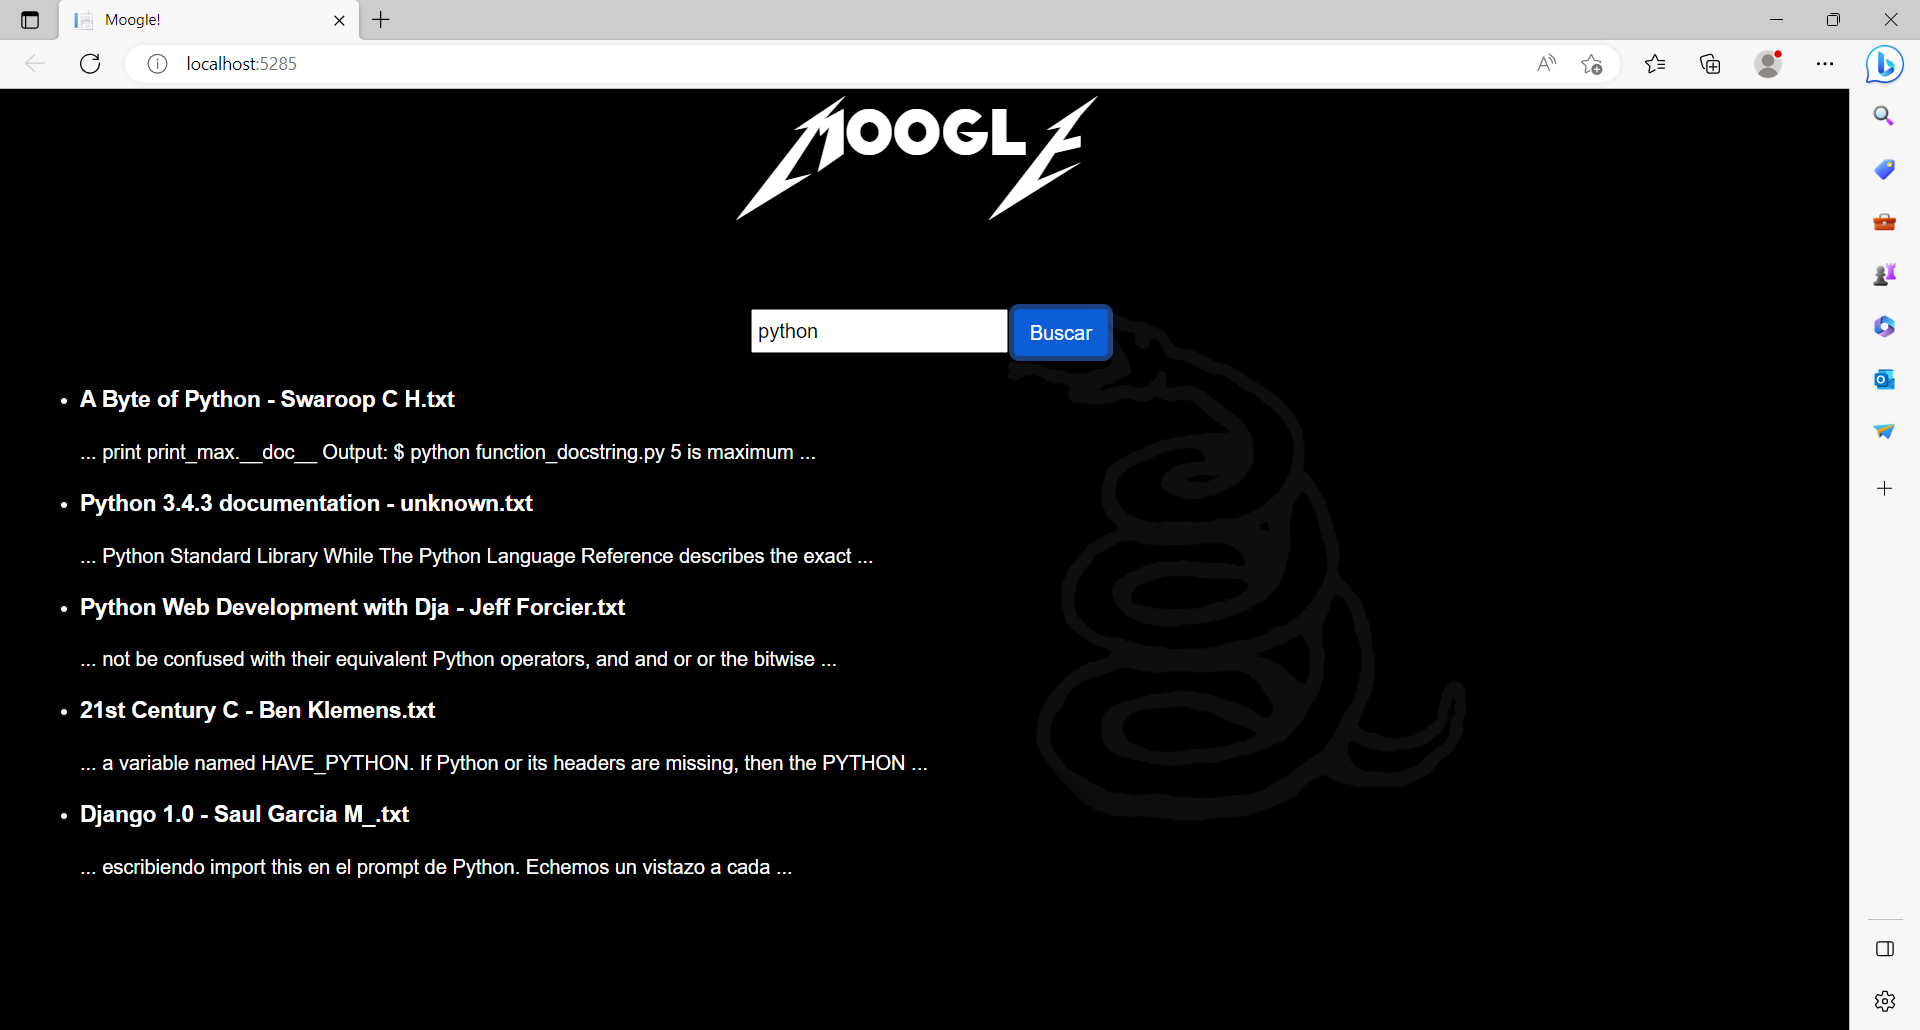
\includegraphics[width=6cm]{busqueda2.png}
    \caption{Debajo de cada resultado aparece el snippet}
\end{figure}

\end{frame}

\subsection{Sugerencias}
\begin{frame}[fragile]{Sugerencias}
En caso de que se una palabra que no se encuentre en el directorio entonces se busca
la palabra que contenga mas similar (usando distancia de levenshtein), luego se sustituye esa
posible palabra en la query y se vuelve a realizar la busqueda, obteniendo los
resultados sugeridos.

\begin{figure}[h]
    \center
    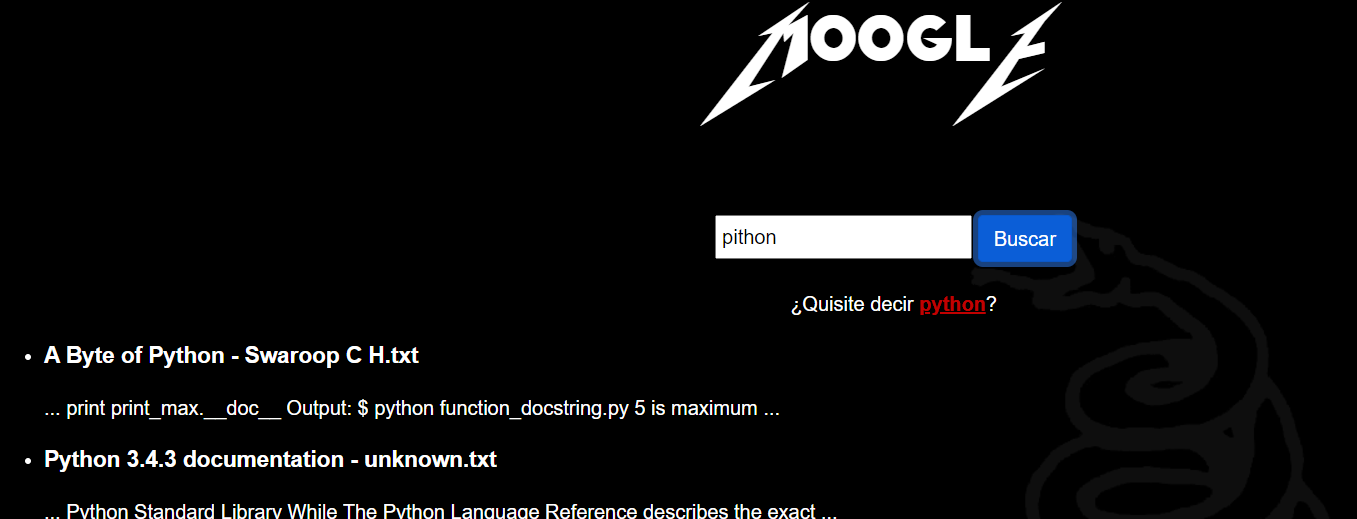
\includegraphics[width=8cm]{sugerencia.png}
    \caption{Ejemplo de Sugerencia}
\end{figure}

\end{frame}
